\documentclass[12pt]{beamer}
\usetheme{JuanLesPins}


\usepackage[frenchb]{babel}
\usepackage[T1]{fontenc}
\usepackage[utf8x]{inputenc}
\usepackage{graphicx}
\usepackage{lmodern}
\author{ALIJATE Mehdi - COUSOT Kevin - NEGROS Hadrien}
\title{Projet GMIN332 : Gestion de données complexes}
%\setbeamercovered{transparent} 
%\setbeamertemplate{navigation symbols}{} 
%\logo{} 
%\institute{} 
%\date{} 
%\subject{} 
\begin{document}

\begin{frame}
\titlepage 


\end{frame}
\begin{frame}
\begin{abstract}
\frametitle{Abstract}
\begin{center}
Accès et consultation de données provenant de différentes solutions de persistance (gros volumes de données distribuées et hétérogènes) au travers d’un démonstrateur.
\end{center}
\end{abstract}
\end{frame}

\begin{frame}
\tableofcontents
\frametitle{Sommaire}


\end{frame}
\section{Introduction et problématique}

\begin{frame}
\begin{block}{Introduction}
Les systèmes NoSQL et les technologies du Web Sémantique sont une alternative aux SGBD classiques.
\end{block}

\begin{block}{Problématique}
\begin{itemize}
\item Données hétérogènes
\item Différents paradigmes de représentation
\end{itemize}
\end{block}



\begin{center}
\textbf{Comment interconnecter ces données?}
\end{center}


\end{frame}
\section{Jeu de données}

\subsection{Description}

\begin{frame}
Nous avons fait appel à trois sources  :
\begin{itemize}
	\item \textbf{INSEE} : COG,  les régions, les départements, les arrondissements, les cantons et les communes, ISF.
	\item \textbf{Geonames} :  de nombreuses informations telles que : noms de lieux géographiques, population, code postale...
	\item \textbf{data.gouv.fr} :  résidences de tourisme classées en France.
\end{itemize}




\end{frame}
\subsection{Schéma}

\begin{frame}
\begin{center}
	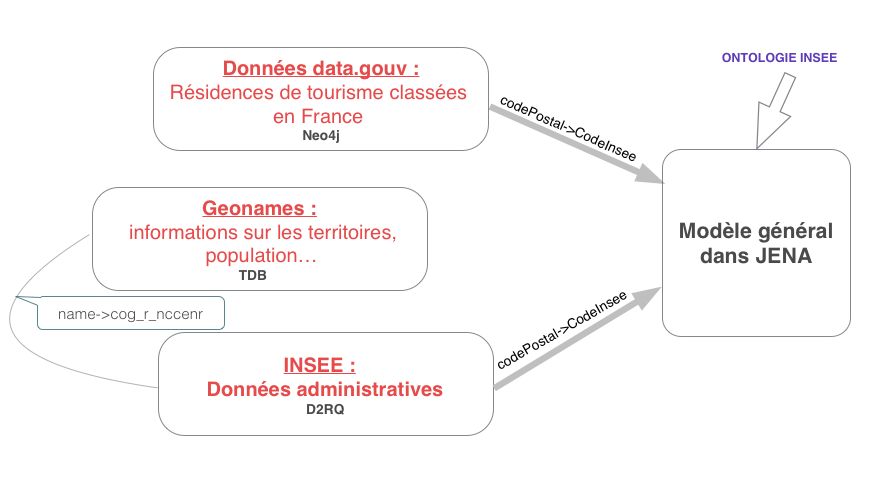
\includegraphics[scale=0.38]{interconnexion.png} 
	
	\label{fig_interconnexion}
\end{center}

\end{frame}
\section{Différents modèles de représentation des données}


\subsection{Modèle relationnel}

\begin{frame}
\frametitle{Modèle relationnel}
\begin{itemize}
\item C'est largement le paradigme le plus utilisé.
\item Les données sont représentées par des tuples.
\item Les contraintes assurent la cohérence et les liens sur les données.
\item Le SGBD que nous avons choisi est \textbf{MySQL}
\end{itemize}
\begin{block}{D2RQ}
D2RQ nous permet de manipuler des données relationnelles comme des triplets RDF.
\end{block}




\end{frame}
\subsection{Triple Store}
\frametitle{Triple Store}
\begin{frame}
\begin{itemize}
\item Un Triple Store est une base de donnée NoSQL conçue pour stocker des triplets RDFs.
\item La consultation des données se fait avec le langage de requête \textbf{Sparql}
\end{itemize}

\begin{block}{TDB}
TDB est une solution de persistance pour les données RDFs.
\end{block}
\end{frame}
\subsection{Base de donnée orientée graphe}

\begin{frame}
\frametitle{BDD orientée graphe}
\begin{itemize}
\item Une base de données orientée graphe est une BDD NoSQL utilisant la théorie des graphes.
\item Pas besoin de schéma, les relations sont des objets de premier ordre.
\end{itemize}

\begin{block}{Neo4j}
La base de donnée orientée graphe que nous avons décidé d'intégré est \textbf{Neo4j}
\end{block}



\end{frame}
\subsection{Base de donnée orientée colonne}
\begin{frame}
\frametitle{BDD orientée colonne}
\begin{itemize}
\item C'est une base de données qui stocke les données sous forme de colonnes.
\item L'intérêt est de sérialisé les colonnes les unes après les autres
\end{itemize}

\begin{block}{Hbase}
La base de donnée orientée colonne que nous avons décidé d'intégré(à la base) est \textbf{Hbase}
\end{block}
\begin{center}
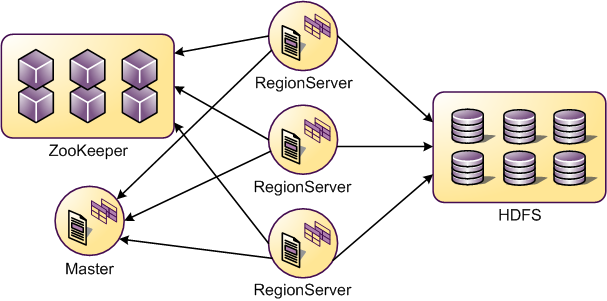
\includegraphics[scale=0.3]{hbase-shema.png} 

\label{fig_hbase}
\end{center}

\end{frame}
\section{Application}

\subsection{L'API Jena}

\begin{frame}
\begin{center}
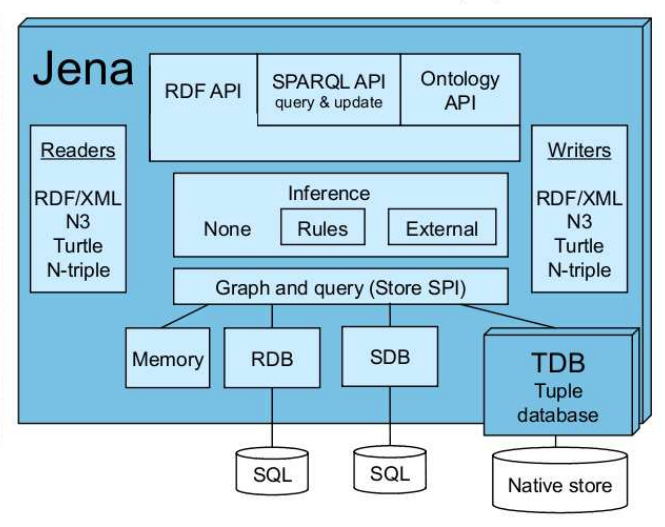
\includegraphics[scale=0.4]{archi_jena.jpeg} 

\label{fig_jena}
\end{center}



\end{frame}
\subsection{Requêtage SPARQL}

\begin{frame}
\frametitle{SPARQL}
\begin{itemize}
\item C'est le language de requêtage sur les données RDFs.
\item SPARQL fonctionne par recherche d'homomorphismes du sous-graphe défini dans la requête vers la BDD.
\item ARQ est le moteur de requêtes SPARQL de JENA, celui-ci y ajoute diverses fonctionnalités telles que les agrégateurs.
\end{itemize}

\end{frame}

\subsection{Architecture de l'application}
\begin{frame}
\frametitle{Architecture}
\begin{center}
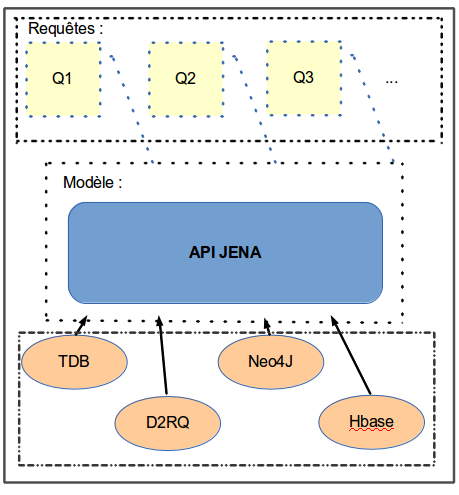
\includegraphics[scale=0.4]{archi_appli.png} 

\label{fig_appli}
\end{center}

\end{frame}
\section{Démonstration}

\begin{frame}

\begin{center}
\huge Démonstration

\end{center}
\end{frame}
\section{Discussion et conclusion}

\begin{frame}


\frametitle{Discussion}
\begin{itemize}
\item Distribution des données sur des sites différents.
\item Ne pas utiliser une bdd embarquée mais l'API REST.
\item Choisir des données plus facilement interconnectables.
\end{itemize}
\begin{block}{Difficultés}
\begin{itemize}
\item Quelques difficultés techniques.
\item Choix des données : interconnection.
\end{itemize}
\end{block}
\end{frame}
\begin{frame}


\frametitle{Conclusion}
Ce projet nous a permis :
\begin{itemize}
\item Expoler les différents solutions NoSql.
\item Familiariser avec l'API Jena.
\item Comprendre l'intérêt d'un modèle commun pour des données hétérogènes. 
\end{itemize}

\end{frame}


\end{document}